\documentclass[12pt,letterpaper, onecolumn]{exam}
\usepackage{amsmath}
\usepackage{amssymb}
\usepackage{commath}
\usepackage{physics}
\usepackage{multirow}
\usepackage{float}
\usepackage{relsize}
\usepackage{tikz}
\usepackage[lmargin=71pt, tmargin=1.2in]{geometry}  %For centering solution box
\usepackage{clrscode}
\usepackage{listings}
\usepackage{xcolor}
\usepackage{pdfpages}
\usepackage{enumitem}
\definecolor{codegreen}{rgb}{0,0.6,0}
\definecolor{codegray}{rgb}{0.5,0.5,0.5}
\definecolor{codepurple}{rgb}{0.58,0,0.82}
\definecolor{backcolour}{rgb}{0.95,0.95,0.92}
\usetikzlibrary{arrows.meta}
\usetikzlibrary{patterns}
\graphicspath{ {./images/} }

\lstdefinestyle{mystyle}{
    backgroundcolor=\color{backcolour},   
    commentstyle=\color{codegreen},
    keywordstyle=\color{magenta},
    numberstyle=\tiny\color{codegray},
    stringstyle=\color{codepurple},
    basicstyle=\ttfamily\footnotesize,
    breakatwhitespace=false,         
    breaklines=true,                 
    captionpos=b,                    
    keepspaces=true,                 
    numbers=left,                    
    numbersep=1pt,                  
    showspaces=false,                
    showstringspaces=false,
    showtabs=false,                  
    tabsize=2
}

%\lstset{style=mystyle}
\lhead{CAP 5610 Assignment \#2 Solution\\}
\rhead{Arman Sayan\\}
% \chead{\hline} % Un-comment to draw line below header
\thispagestyle{empty}   %For removing header/footer from page 1

\begin{document}

\begingroup  
    \centering
    \LARGE CAP 5610\\
    \LARGE Assignment \#2 Solution\\[0.5em]
    \large \today\\[0.5em]
    \large Arman Sayan\par
\endgroup
\rule{\textwidth}{0.4pt}
\bracketedpoints   %Self-explanatory
\printanswers
\renewcommand{\solutiontitle}{\noindent\textbf{Ans:}\enspace}   %Replace "Ans:" with starting keyword in solution box
\qformat{\large \textbf{\thequestion \quad \thequestiontitle \quad [\thepoints] \hfill}}
\renewcommand{\thepartno}{\arabic{partno}}
\renewcommand{\partlabel}{\thepartno.}

\begin{questions}
    \titledquestion{Types of Attributes}[10]
    
    Classify the following attributes as nominal, ordinal, interval, ratio. \textbf{\underline{Explain why}}.

    \begin{enumerate}[label=(\alph*)]
        \item Rating of an Amazon product by a person on a scale of 1 to 5
        \item The Internet Speed
        \item Number of customers in a store.
        \item UCF Student ID
        \item Letter grade (A, B, C, D)
    \end{enumerate}
    
    \begin{solution}
        Write answer
    \end{solution}

    \pagebreak

    \titledquestion{Distance/Similarity Measures}[20]

    Given the four boxes shown in the following figure, answer the following questions. In the 
    diagram, numbers indicate the lengths and widths and you can consider each box to be a vector 
    of two real numbers, length and width. For example, the top left box would be (2,1), while the 
    bottom right box would be (3,3). Restrict your choices of similarity/distance measure to 
    Euclidean distance and correlation. \textbf{\underline{Please explain your choice}}.

    \begin{figure}[h]
        \centering
        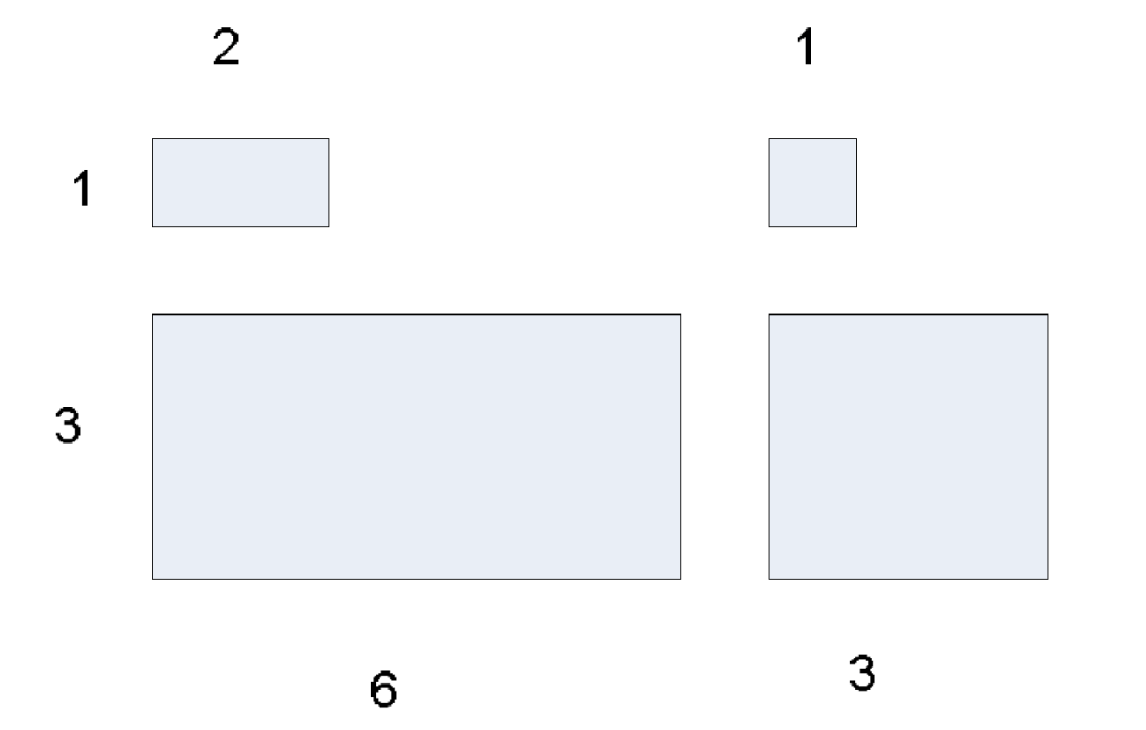
\includegraphics[width=0.65\textwidth]{boxes.png}
    \end{figure}

    \begin{parts}

        \part[10] Which proximity measure would you use to group the boxes based on their
        shapes (length-width ratio)?

        \begin{solution}
            Write answer
        \end{solution}

        \part[10] Which proximity measure would you use to group the boxes based on their
        size?

        \begin{solution}
            Write answer
        \end{solution}
        
    \end{parts}

    \pagebreak

    \titledquestion{Coding Question}[20]

    Please write a Python code to calculate Cosine similarity, and Euclidean distance using NumPy. 
    The input can be two randomly generated vectors or fixed vectors written by yourself. 
    Note that: For Coding Questions, please \textbf{\underline{do not}} directly call linear regression and non-linear 
    regression built-in functions in existing library packages such as scikit-learn. You may call basic 
    computation functions built in Numpy.

    \begin{solution}
        Write answer
    \end{solution}

    \pagebreak

    \titledquestion{Coding Question}[25]

    Please implement a Linear Regression to find the best linear model for the provided
    linear data. Please plot the result using "matplotlib.pyplot".

    Note that

    \begin{enumerate}[label=(\arabic*)]
        \item The linear model is in the following format $Y=mX+c$
        \item Use MSE as the loss function
        \item You may use “pandas” to read the csv file and load the values into two vectors $X$ and $Y$.
        \item Use Gradient Descent for the training. You may choose fixed learning rate (such as
        0.0001) and epochs (such as 1000) without considering mini-batch.
        \item The result will look like the following image.
    \end{enumerate}

    \begin{figure}[h]
        \centering
        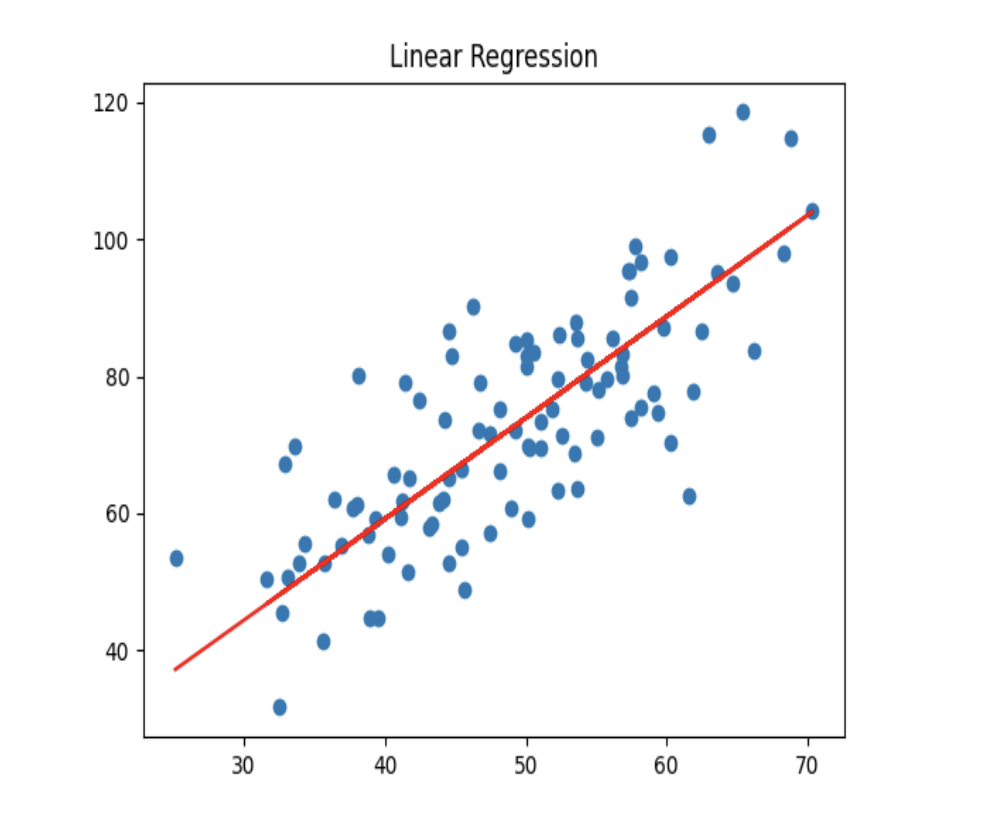
\includegraphics[width=0.65\textwidth]{linear.png}
    \end{figure}

    \begin{solution}
        Write answer
    \end{solution}

    \pagebreak

    \titledquestion{Coding Question}[25]

    Please implement a non-linear regression to find the best cubic function model for the 
    provided non-linear data. Please plot the result, too.

    \begin{enumerate}[label=(\arabic*)]
        \item The cubic function is in the following format: $Y=aX^3+bX^2+cX+d$
        \item Use MSE as the loss function.
        \item Use Gradient Descent for the training. You may choose fixed learning rate (such as
        0.000001 (1e-6)) and epochs (such as 10000) without considering mini-batch. It may take
        10-15 seconds to finish the running for 10000 steps. Please be patient.
        \item The result will look like the following
    \end{enumerate}

    \begin{figure}[h]
        \centering
        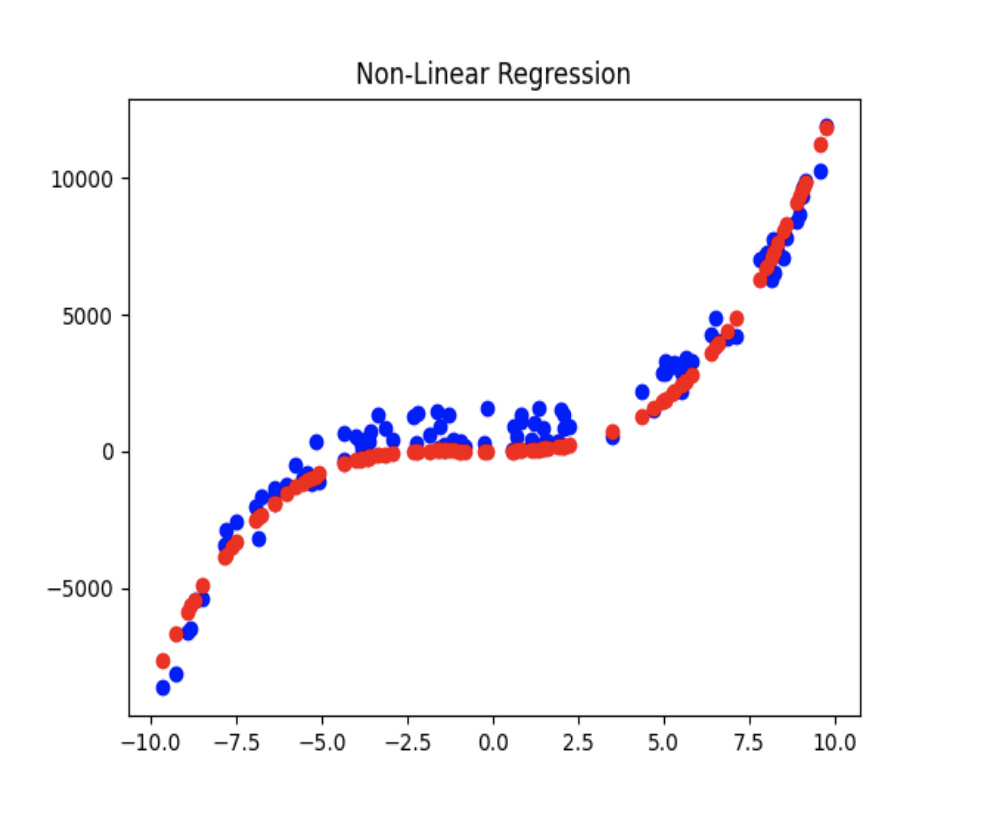
\includegraphics[width=0.65\textwidth]{non-linear.png}
    \end{figure}

    \begin{solution}
        Write answer
    \end{solution}

    \pagebreak
    
\end{questions}

\begin{appendix}
    \centering
    %\begin{flushleft}  
    %  \section{Appendix}
    %  \includepdf[pages=-]{CAP_5610_Assignment_1_Solution_Arman_Sayan_1.pdf}
    %\end{flushleft}
\end{appendix}

\end{document}